\section{Analysis}
\label{analysis}

\begin{figure*}[th!]

    \centering
    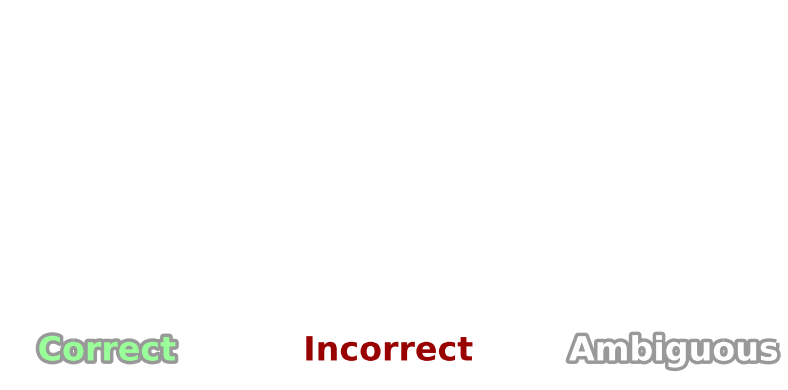
\includegraphics[width=0.5\textwidth, trim={0 0 0 3.3in},clip ] {figures/labels.png}\\
    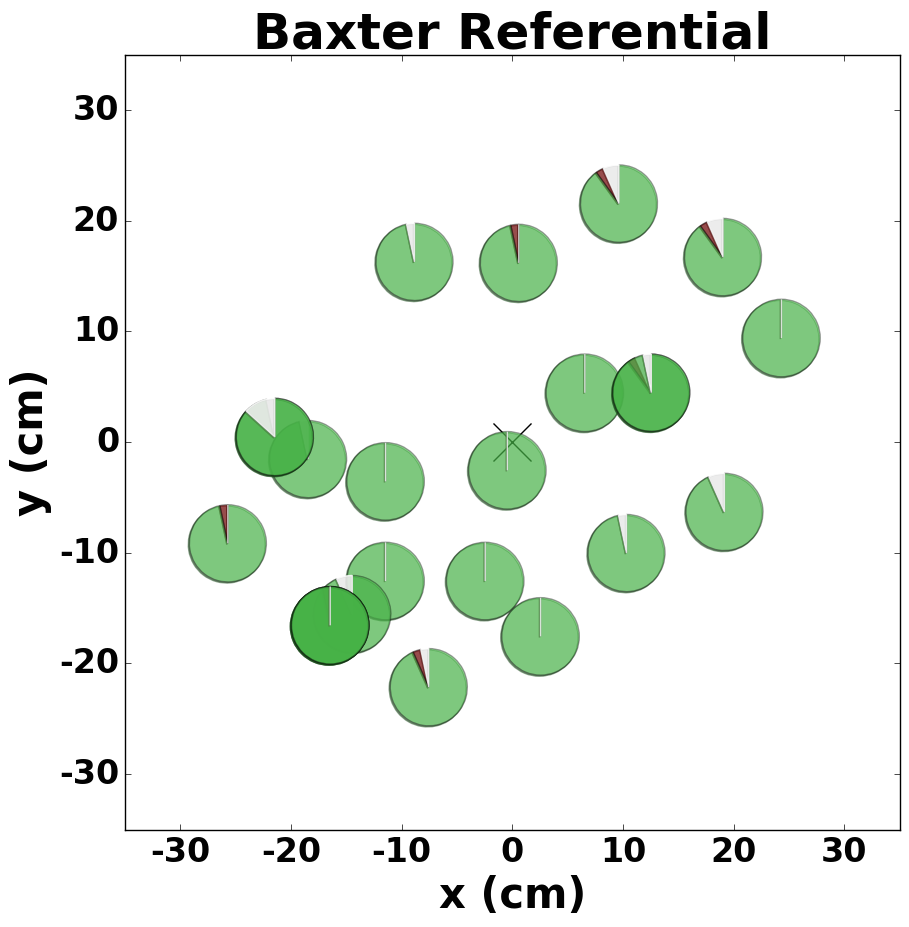
\includegraphics[width=0.325\textwidth ] {figures/baxter_Referential_.png}
    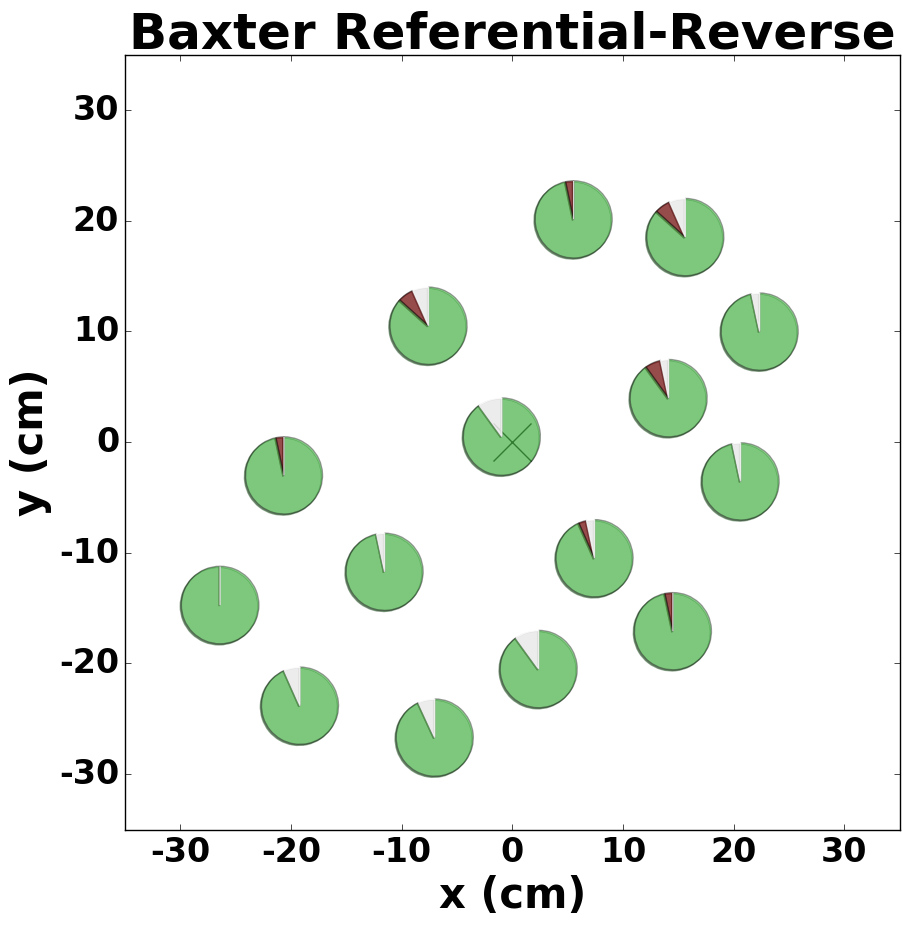
\includegraphics[width=0.325\textwidth ] {figures/baxter_Referential-Reverse_.png}
    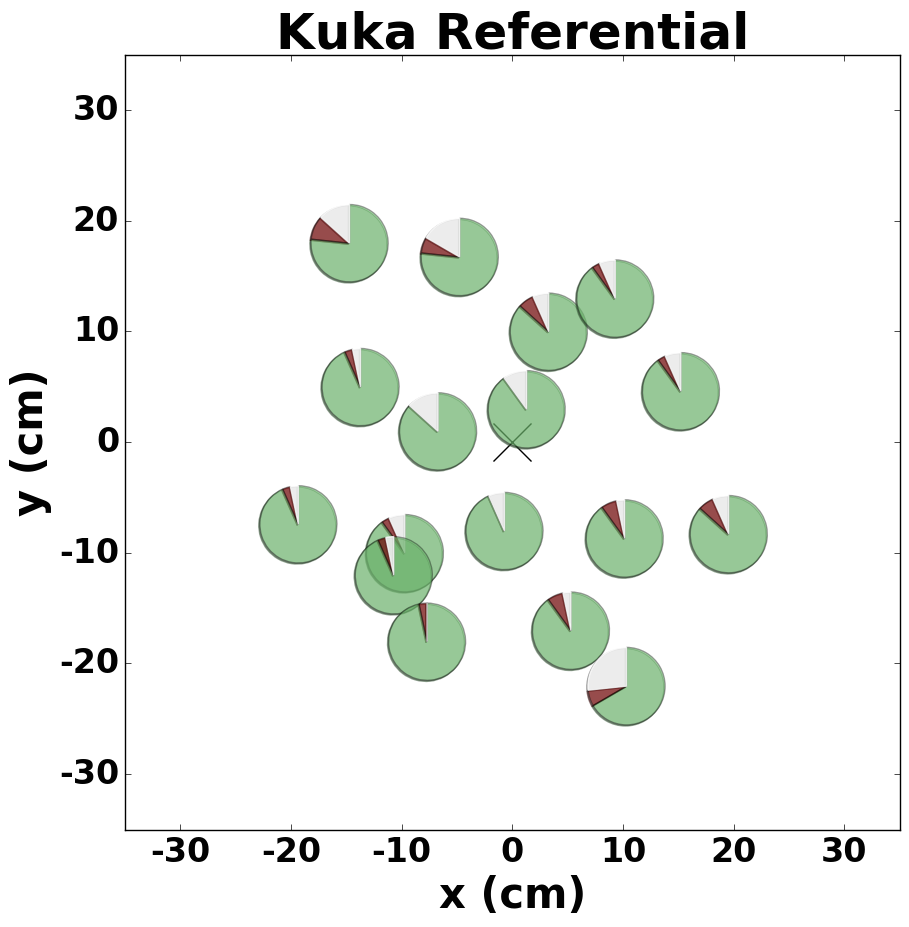
\includegraphics[width=0.325\textwidth ]{figures/kuka_Referential_.png}
    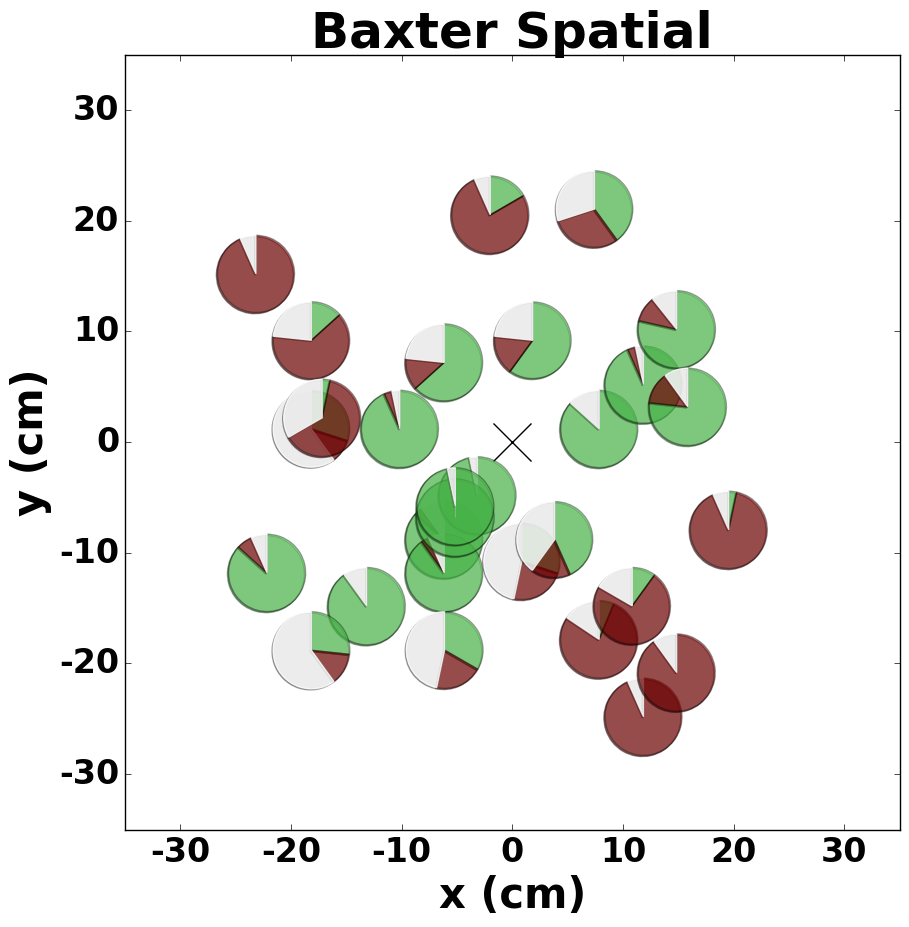
\includegraphics[width=0.325\textwidth ]{figures/baxter_Spatial_.png}
    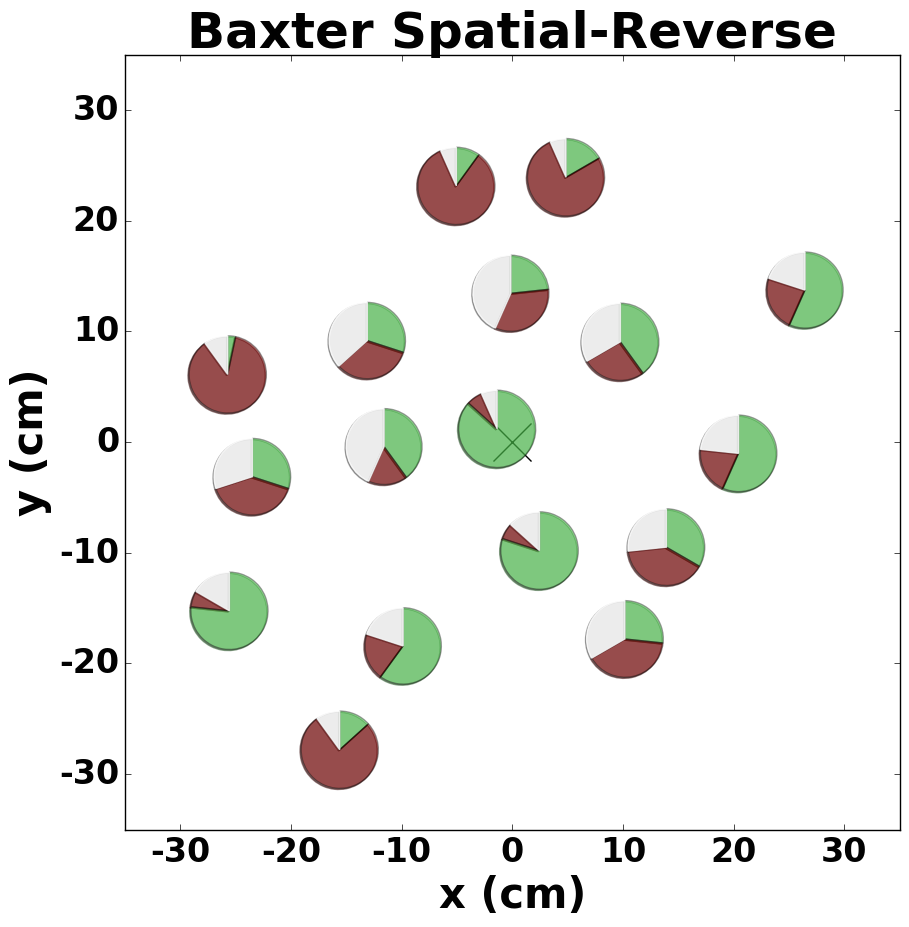
\includegraphics[width=0.325\textwidth ]{figures/baxter_Spatial-Reverse_.png}
    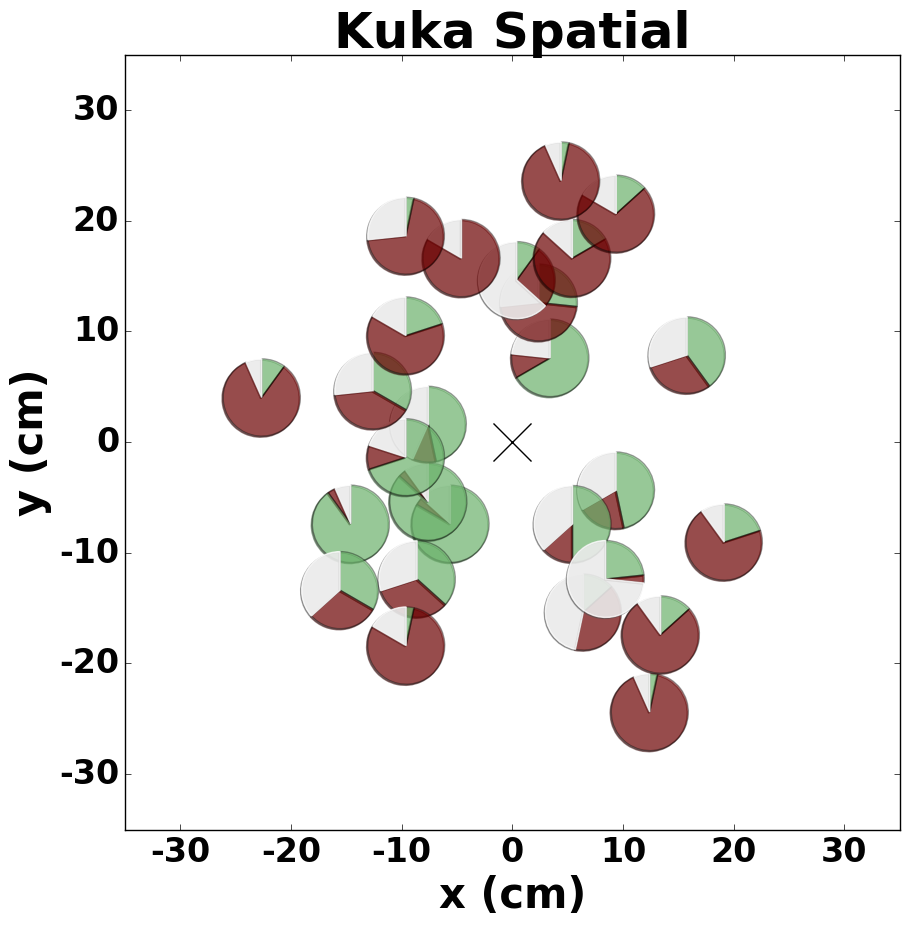
\includegraphics[width=0.325\textwidth ]{figures/kuka_Spatial_.png}
    \caption{The aggregated results from the referential versus spatial trials for the \textit{Baxter} and \textit{Kuka} robots. The locations of the responses correspond to the center of the circles, and are plotted in the coordinate frame centered at the position of the pointing action, marked with $\times$. The circles show the fraction of correct (grey), incorrect(black) and ambiguous(white) responses.}
    \label{fig:aggregatesimple}
\end{figure*}

\paragraph{Referential vs Locating}
We study how varying the target of the pointing action from a referent object to a part of the space changes the interpretation of the pointing action by comparing the interpretation of the position of the pointing action $x^*$ in each condition. 

Figure~\ref{fig:aggregatesimple} shows the results of the experiment. The plot shows the spread of \textit{correct, incorrect, ambiguous} responses over the sampled positions about the location of a referential, and spatial pointing action. The referential data demonstrates the robustness of the interpretation. Most of the responses were overwhelmingly \textit{`correct'}, for both robots in interpreting a referent object in the \textit{pick} part of a pick-and-place task. The spatial pointing shows a much higher sensitivity to an accuracy of $x^*$ with respect to the true final placement. This comes up as a larger incidence of \textit{`incorrect'} and \textit{`ambiguous'} responses from the human subjects. This trend is true for the reverse trial as well.

While the study attempts to separate out and measure the critical aspects of the interpretation of robotic pointing actions some ambiguities like those arising out of perspective of the camera being projected onto a simulated 2D video or image are unavoidable. We suspect that the observed stretch of \textit{'correct'} responses in spatial trials is due to perspective.

To test our hypothesis, we performed a Chi-squared test and compared the proportion of \textit{correct}, \textit{incorrect} and \textit{ambiguous} responses in referential and spatial trials. The results of the test shows that these two classes are statistically significantly different ($\chi^2= 13.89, p = 0.00096$).

To study if we are observing the same effects in the results of the reverse trial, no speech trial and the Kuka trial, we ran an equivalence test on the third hypothesis following the two one-sided tests method as described in \cite{lakens2017equivalence}, where each test is a pooled z-test with no continuity
correction with a significance level of 0.05. We found that changing the robot, removing the speech and changing the direction of the pointing action does not make a difference in the interpretation of spatial pointing and referential pointing within any margin that is less than 5\%.


\begin{table}[h]
% \vspace{-0.3in}
\label{tab:naturaltrial}
\begin{tabular}{lllll}
          &               & correct     & incorrect & ambiguous \\ \hline
unnatural & top           & 12          & 9         & 9         \\
          & \textbf{edge} & \textbf{24} & 2         & 4         \\
          & table         & 2           & 2         & 26        \\ \hline
natural   & \textbf{top}  & \textbf{26} & 3         & 1         \\
          & edge          & 9           & 11        & 10        \\
          & table         & 7           & 13        & 12        \\ \hline
\end{tabular}
\caption{Results of the unnatural scene and natural scene. (numbers are our of 30) }
\label{tab:natural-unnatural}
\end{table}

\paragraph{Natural vs Unnatural}

As shown in Table~\ref{tab:natural-unnatural} we observed in the natural scene, when the end-effector points towards the edge of the cube that is on top of the stack, subjects place the new cube on top of the stack or on the table instead of the edge of the cube. However, in the unnatural scene, when we explain to subjects that there is no gravity, a majority agree with the final image that has the cube on the \textit{edge}.






\paragraph{Different verbs}
The results of the Chi-squared test shows that in spatial trials when we replace \textit{put} with \textit{place}, \textit{push} and \textit{move}, the differences of the distributions of \textit{correct}, \textit{incorrect} and \textit{ambiguous} responses are not statistically significant ($\chi=0.2344 $, $p = 0.971$). The coefficients of the multinomial logistic regression model and the p-values also suggest that the differences in judgements 
with different verbs are not statically significant ($b<0.0001$ , $p>0.98$).


\begin{figure}[h!]
    \centering
    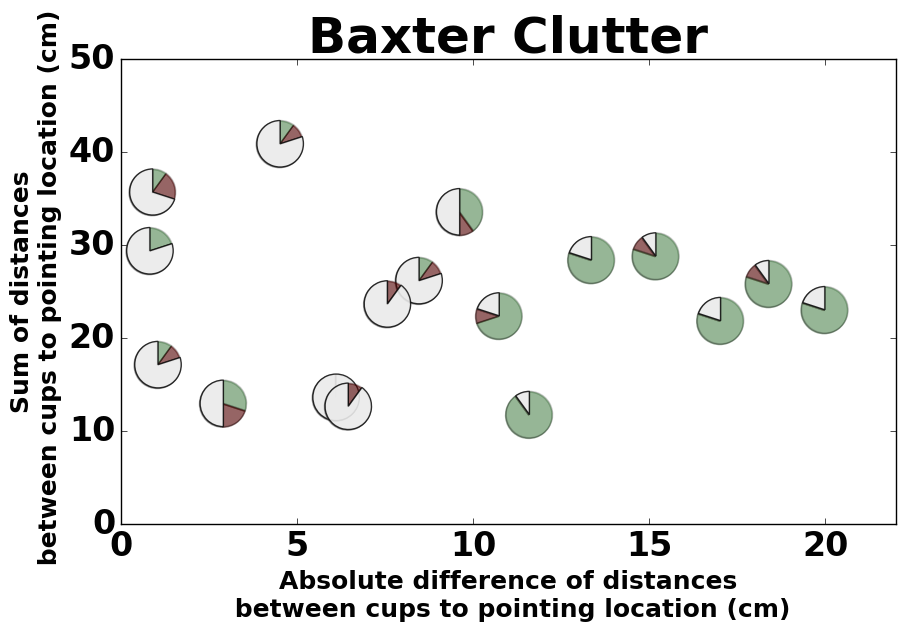
\includegraphics[width=\linewidth]{figures/baxter_Clutter_granular.png}
    \caption{The scatter plot represents the spread of responses where human subjects chose the \textit{nearer cup} (green), \textit{farther} cup (red), and ambiguous (white). The \textit{x-axis} represents the absolute difference between the distances of each cup to the locations of pointing, the \textit{y-axis} represents the total distance between the two cups.}
    \label{fig:cluttered}
\end{figure}
\paragraph{Cluttered}
The data from these trials show how human subjects select from the two candidate target objects on the table. Since the instructions do not serve to disambiguate the target cup, the collected data reflects what was deemed as the \textit{correct} target by the observers. 
Figure~\ref{fig:cluttered} shows the fraction of responses for every experimental trial that recorded the nearer (green) cup as correct, versus the farther cup (red). The white shaded fractions of the pies show the fraction of responses where subjects found the action ambiguous.

As we can see in Figure~\ref{fig:cluttered}, the higher is the absolute difference of centers of distances from the center, the more likely it is that subjects pick a mug (green or red) as opposed to the \textit{ambiguous} choice. That is when the two mugs were very close, almost next to each other (less than 10 cm apart), majority of subjects chose the \textit{ambiguous} option. When one of the cups was significantly closer than the other one (greater than 10cm apart on the X-axis) the subjects preferred the closer (green) cup. 







When the target is not very close to the distractor, and when the pointing finger points towards $x^*$ on the table that is closer to one mug, subjects picked the mug that was the correct target of the pointing action more often than the incorrect one. This was true for all of the cases in our dataset. 


